\documentclass[12pt, letterpaper, twoside]{article}
\usepackage[sorting=none, backend=bibtex]{biblatex} %Imports biblatex package
\bibliography{ref} %Import the bibliography file
\usepackage[hmarginratio=1:1]{geometry}
\usepackage[utf8]{inputenc}
\usepackage{graphicx}
\usepackage{hyperref}
\usepackage{subcaption}

\title{Pepper Waiter HRI Project}
\author{Daniele Appetito 1916560\\
 Salvatore Cognetta 1874383\\
  Simone Rossetti 1900592}
        
\date{September 2021}

\begin{document}

\begin{titlepage}
\maketitle
\end{titlepage}

\tableofcontents

\newpage
    
\newpage
\section{Introduction}

Human Robot Interaction is the study of how one or more humans work with one robots in order to accomplish a goal. The Pepper Waiter project was devised to create such an interaction. 

\

Pepper is a robot created by Softbank Robotics specifically to interact with people. It has tactile, visual, and audio sensors on its body to help a person convey  information in a variety of ways. On top of that it is equipped with an android tablet on its "chest" that can be used for further interaction. 

\

The aim for this project was to create a way for Pepper to interact (whether virtually or physically) with people in an environment of our choice. 

In this project we decided to create a program that allowed to use the Pepper in a bar or restaurant environment to take an order instead of a human. This idea came to us by thinking of the current global situation and how the less human-to-human contact there is, the better. As such we decided to create a way to adhere to the social distancing norms by removing interaction with a human waiter. 


\


\section{Inspiration and Research}

The main source of inspiration for the choice of this project was the currently ongoing COVID-19 pandemic, and the idea that we wanted to create a way to keep a somewhat social interaction while respecting social distancing norms. We did initially research other papers however, one of which was about the use of robots to mimic colloquial accents \cite{10.3115/976909.979652} in different languages to make a person feel more "at home", and ease the communication. A second paper we looked at involved the use of anthropomimetic robots \cite{Wittmeier2013TowardAR} (i.e. robots that mimic not only th skeletal, but also the muscular structure of a human). A third paper we saw had to do with the portraying of emotions in a robot's face \cite{BREAZEAL2003119}. 

\

Some further research made us realise that we would need to have an exceedingly more complex robot in order to fully incorporate all the functions we studied above. As such we went over the more necessary functions that could be implemented and used by Pepper.

Because the aforementioned Softbank Robotics robot does not have any moving facial features (e.g. eyebrows, upper/lower lips, cheekbones, etc) we decided to ignore the facial features and instead incorporate a sort of emotion through words, such as using exclamation marks, "please" and "thank you", etc. The same reasoning was done for the dialect and anthropomimetics, which cannot realistically be fully implemented on a Pepper robot, instead we decided to use multiple languages to help with communication. Seeing as Pepper has a somewhat similar physical structure to a human (humanoid head, humanoid hands, torso) we decided that it was a good enough attempt at mimicking human posture.

\

After a final research and consideration we decided that creating a robot waiter would be the best way to portray all of our ideas into a single project.
In the problem we analysed earlier we concluded that we wanted a way to allow safe interactions in restaurants/bars that adhered to the social distancing norms imposed due to the current global pandemic. To solve this problem we decided to create a robot waiter that would help serve people in a restaurant. This solves the problem partially as it gets rid of a whole interaction step in the business by replacing it with a machine incapable of contracting diseases (given that it is kept clean and sanitised often). 

\section{Implementation}
Different tools and API are used in order to create human interactions with a Pepper real robot or simulator, like:

\begin{itemize}
	\item Softbank SDK;
	\item Naoqi softwares;
	\item MODIM - Multi-modalInteraction Manager.
\end{itemize}

All of the tools are described in the following paragraphs.\\

\subsection{Softbank SDK simulator}
The Softbank company, which produces Pepper robots, has made avaible an SDK which allows to connect to a real robot or to create a simulation of the robot using Android Studioa application (\href{https://qisdk.softbankrobotics.com/sdk/doc/pepper-sdk/index.html}{Softbank SDK}). Because of Covid constraints, it was not possible to use directly the Pepper robot, placed in the laboratories of DIAG-University of La Sapienza: for this reason the simulatotion mode is was used.\\

This simulator gives the opportunity of visualize the movements, the dialogs and the interactions that the robot has with people.

\begin{figure}[htbp]
	\centerline{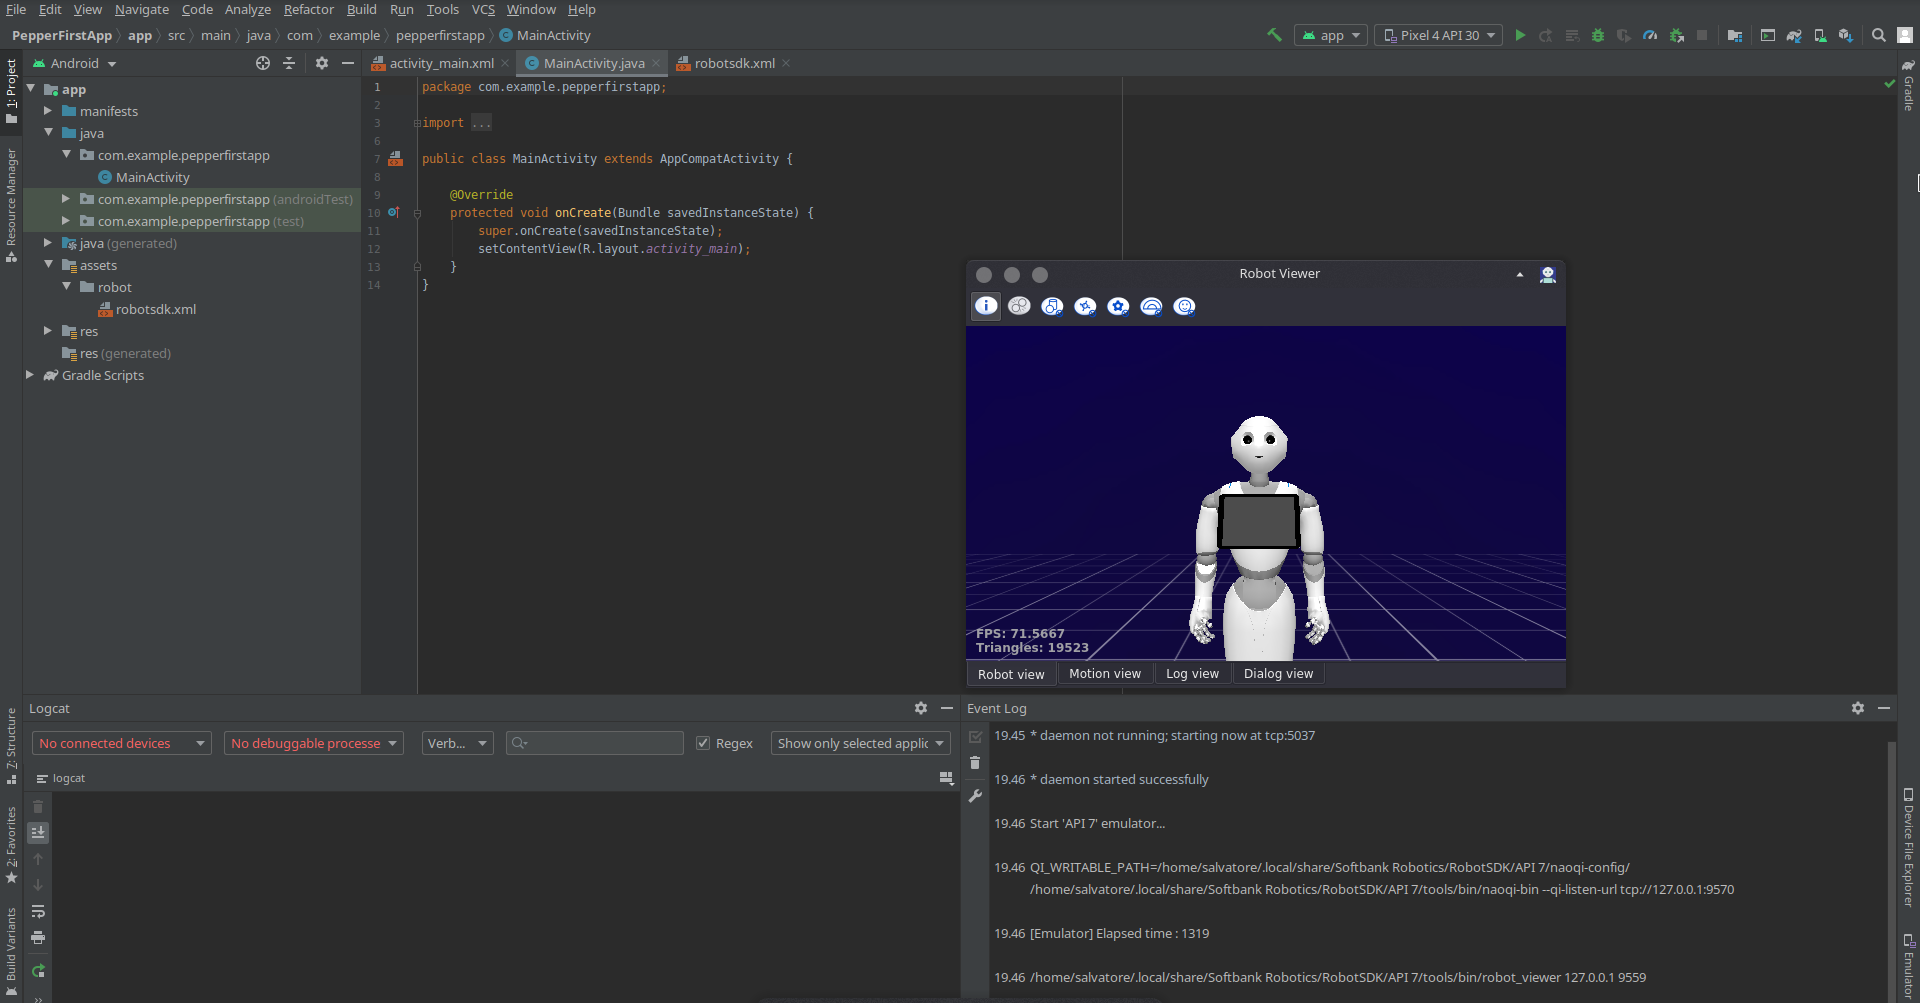
\includegraphics[scale=.3]{img/pepperSDK.png}}
	\caption{Pepper simulator in Android Studio.}
	\label{fig:android_sdk}
\end{figure}

Therefore, to be able to interact and communicate with Pepper, this simulator is used as a client interface, which is connected to a docker image containing the \verb|naoqi| Operative System, containing all the tools and softwares used to run and operate the robot itself.\\
In the simulator, as can be seen from the figure \ref{fig:android_sdk}, there is also a tablet on the chest of the robot. This tablet can be virtualized through another library, modim, later detailed.

\subsection{Naoqi - Pepper tools}
As said before, the OS of Pepper is virtualized thanks to a docker image that is running on our host systems (For further references see the following \href{https://bitbucket.org/iocchi/hri_software/src/master/}{Git Repository}).\\
Once inside the docker image the \verb|naoqi| software must be started in order to initialize and register all services of Pepper, like Dialogs, TextToSpeech, SpeechRecognitrion and more.\\

\begin{figure}[htbp]
	\centerline{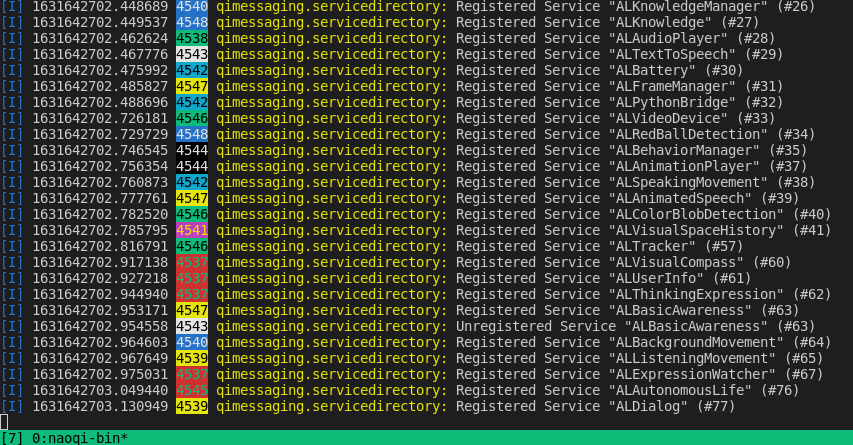
\includegraphics[scale=.6]{img/naoqi.png}}
	\caption{Naoqi SDK: overview of service registered on start.}
	\label{fig}
\end{figure}

This gives us the possibility of command Pepper, indeed inside the docker image different tools are present, with wich one can set some robot parameters like joint angles and the posture, or simulate an input on a sensor like the approach of an human being or a person that talks with Pepper.\\

Beyond the already presented tools, obviously scripts created from us can be runned inside naoqi, in order to set the behaviour of the robot. These scripts can be put inside a shared falder between the host system and the docker image (the directory is \verb|/home/pc_name/playground|). Inside this directory the Pepper Waiter softwares are positioned and developed .

\subsection{Modim}
Like described before, the app running on Pepper's tablet can be virtualized through antoher library called Modim (For further references see the following \href{https://bitbucket.org/mtlazaro/modim.git}{Git Repository})\\

\begin{figure}[htbp]
	\centerline{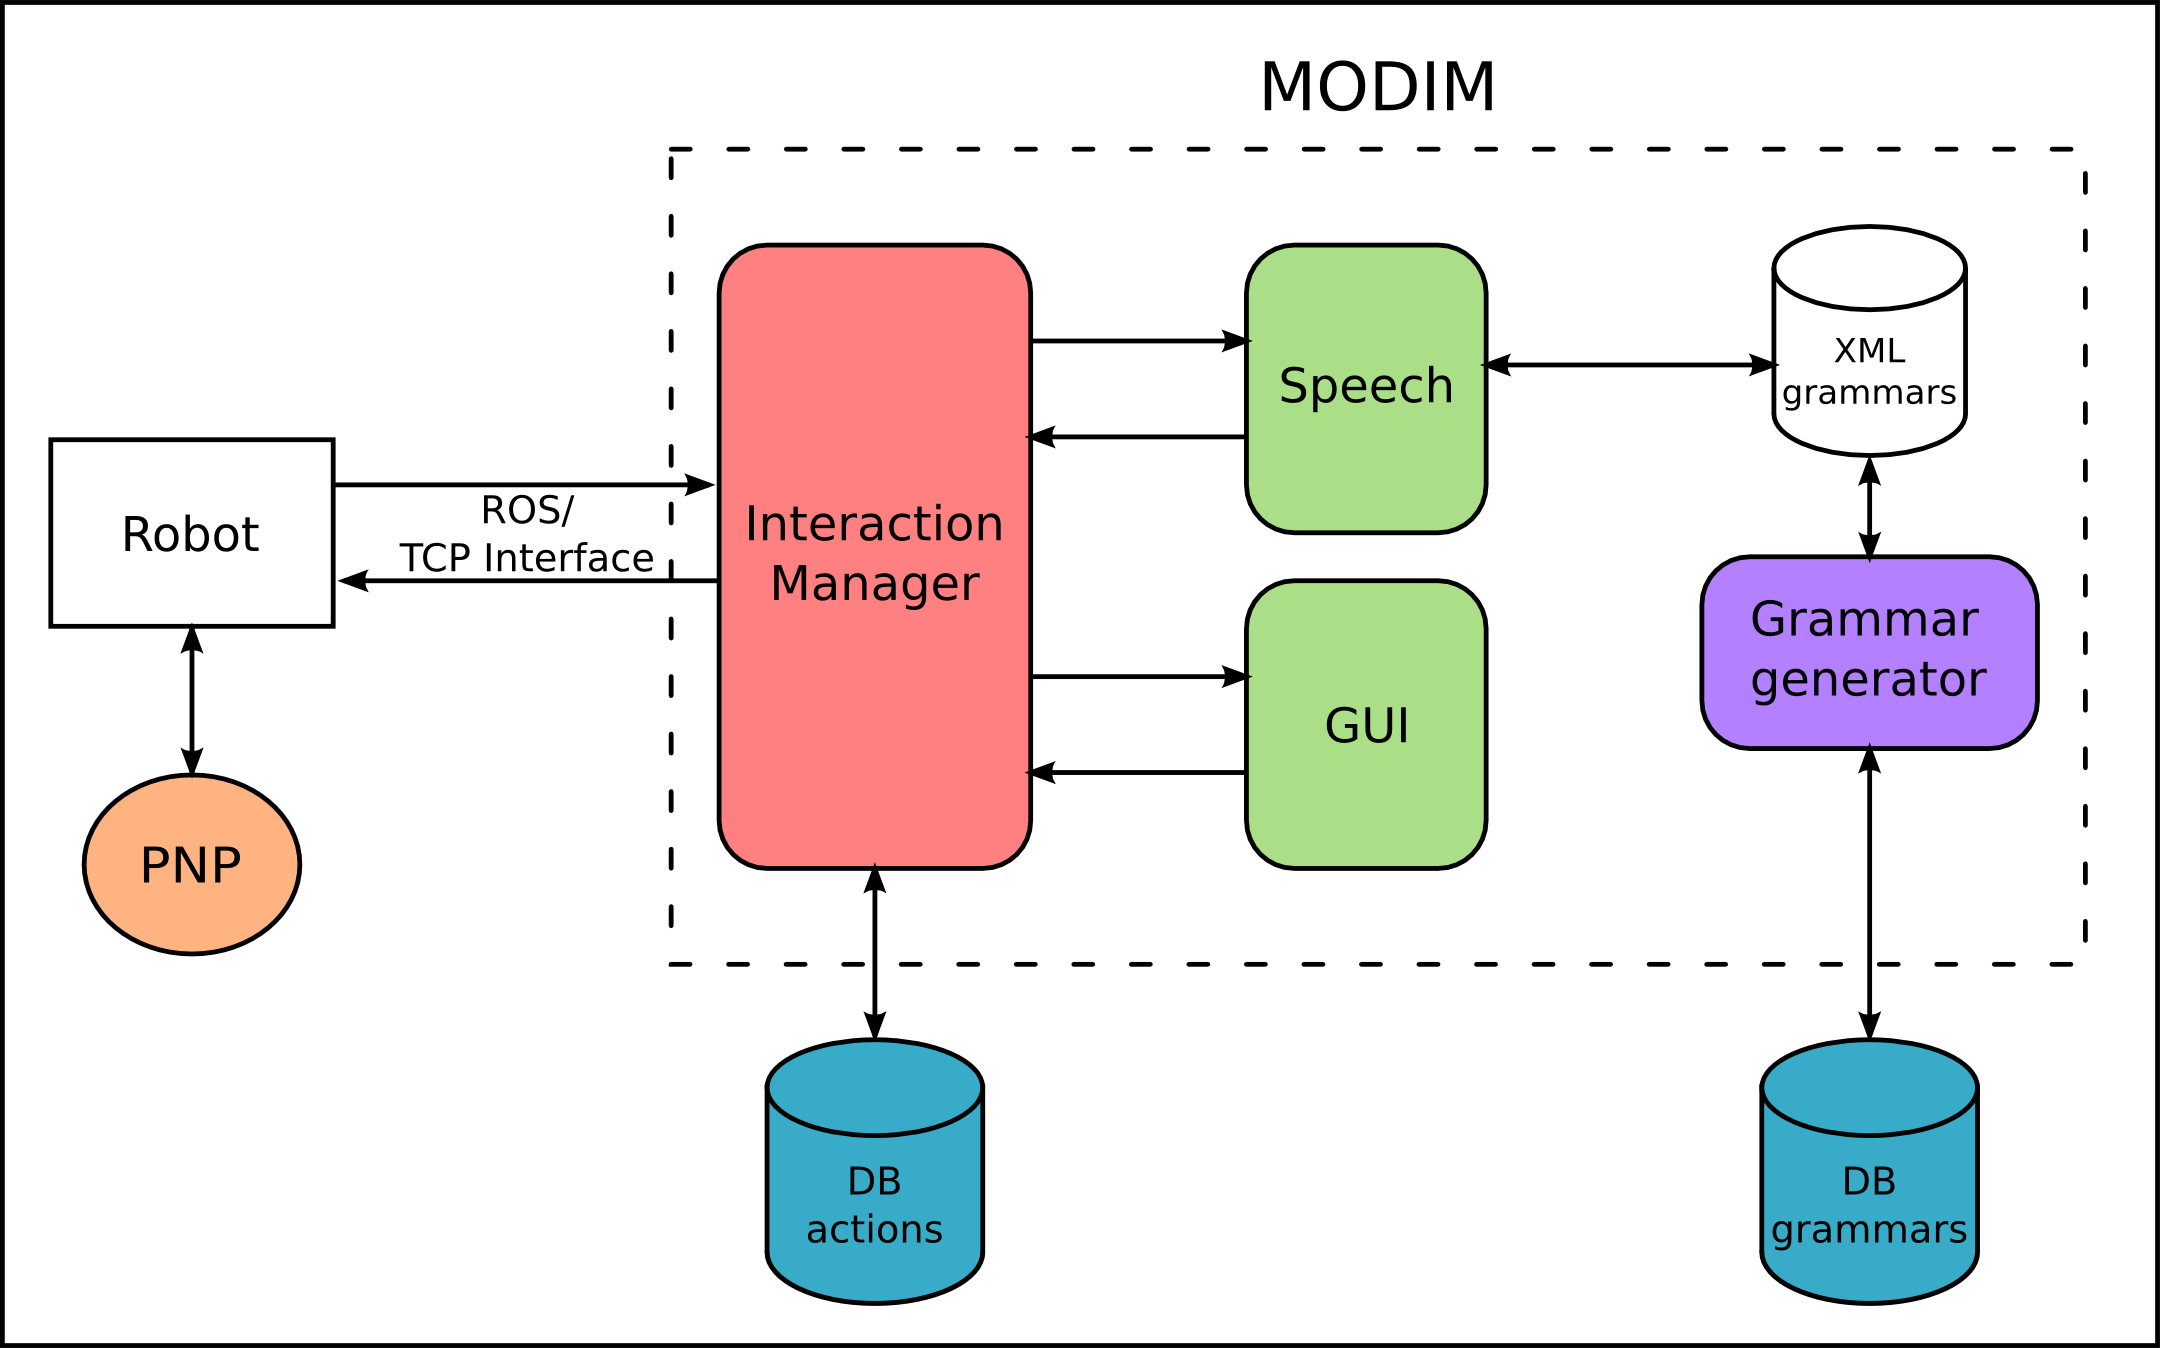
\includegraphics[scale=.6]{img/modim.png}}
	\caption{ Multi-modal Interaction Manager software architecture.}
	\label{fig}
\end{figure}

The Multi-modalInteraction Manager (MODIM), the Graphical User Interface (GUI) and the speech system allow the use of different modalities for the output and input of information from the robot to the user and viceversa. The output modalities considered are the use of texts, images or videos using the GUI or by voice using the speech synthesis. Input modalities are the touch-screen (i.e., with the use of buttons on the GUI) or spoken inputs interpreted by the speech recognizer.\\

Therefore, after connecting the Interaction Manager with Pepper, thanks to this library the app on the tablet can be simulated on a web browser; the user can interact with this one with buttons present on the GUI, both clicking on them through the web browser and giving spoken input (e.g. simulating them thanks to the \verb|naoqi| software).

\begin{figure}[h]
	\centering
	\begin{subfigure}{.5\textwidth}
	  \centering
	  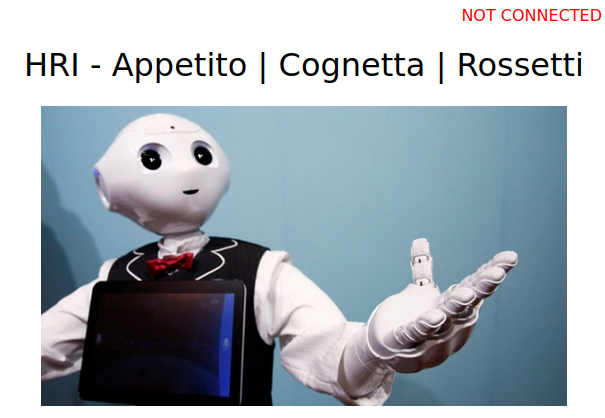
\includegraphics[width=1\linewidth]{img/modim_notok.png}
	  \caption{Modim not connected to Pepper.}
	  \label{fig:sub1}
	\end{subfigure}%
	\begin{subfigure}{.5\textwidth}
	  \centering
	  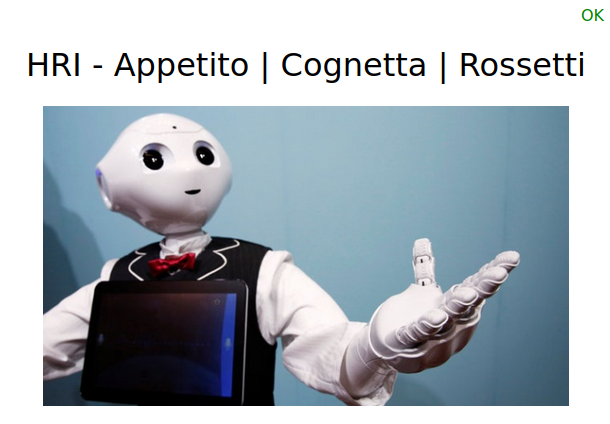
\includegraphics[width=1\linewidth]{img/modim_ok.png}
	  \caption{Modim connected to Pepper.}
	  \label{fig:sub2}
	\end{subfigure}
	\caption{Connection of MODIM to the robot}
	\label{fig:test}
\end{figure}

\newpage

\section{Results}

Pepper Waiter works as a virtual (or physical, although we could only test it virtually) waiter that is designed to welcome customers to a restaurant and take their order, as well as assist them in paying the bill.

\

When a person approaches Pepper, its front sensors will detect an object and greet the customer with a welcome message both on its front tablet, and by voice. From there a customer can choose from a 4 options: "Menu", "Order", "Checkout", and "Review". All of these options being self explanatory and selecting each word will take the customer to a separate screen for the according action. 

\

The "Menu" screen consists of an individual page for each item of the menu (5 in total) where one can read the description, the ingredients, and the price. Pepper will also read the description out loud. After having decided on what to order from the menu the customer can the return to the main page described in the previous paragraph to continue on with the order.

\

In the "Order" screen one can choose any of the 3 available dishes (pizza, nachos, tiramisu) and 2 drinks (water, red wine). After clicking on one of the 5 aforementioned	buttons the customer can then choose the quantity of the food/beverage that they want. Once they are fully ready they can click on "Review Order" to review what they have ordered. From there the customer will have the possibility of altering the order one or confirming it. Once confirmed, the customer will receive an order number that will be then used to recognise the order at checkout. After this the robot will automatically go back to the main menu page, in order to prepare to serve someone else.

\

Once the customer is finished with the food they can then walk over to pepper again and (after being greeted again) can press the "Checkout" button, where a list of the ordered items and the total price will be displayed. In this page one will be able to review their order after stating the order number assigned to them earlier. Once the payment is confirmed the customer can choose to leave a review of the service where they'll have to rate their experience with Pepper on a scale of 1 to 5. 




\section{Conclusion}

We created a program for the Pepper robot designed to interact with humans in a customer-waiter way. The project itself was fun and challenging. One of our greater challenges was docker setup as well as the simulation start on android studio. However, after the initial hickups on starting to use the program, the process was streamlined and entertaining. We learned a lot about android application creations, as well as what Pepper is capable of doing. 

\

Something that would be nice to try in the future is to actually use the program on Pepper itself rather than a simulation. Due to the current pandemic we were not allowed physical access to the robot. I think seeing the program work on a fully functioning Pepper robot live would be the next step in looking at improving the project. One thing that could be done to further improve on this project is create a navigation program that would let Pepper guide you to the desired free table before assisting you with an order. Of course, the most ideal improvements to this experience would be using a robot with a more anthropomimetic figure (i.e. a full human body, which currently do not exist at this level of automation) and with a range of changing facial features, in order to express contempt/happiness. This would allow it to more accurately mimic a real human-to-human interaction.  

\




\newpage

\nocite{*}
\printbibliography[heading=bibintoc,title={References}]
\end{document}